\section{Parabolic Fixed Points}
\sectiontitleframe

\begin{frame}{Attraction vectors}
    \begin{equation*}
        f(z)=\lambda z + \mu z^{p + 1} + \dots
    \end{equation*}
    \begin{itemize}
        \item When $\lambda = 1$, fixed point exhibits both attractive and repulsive properties.
        \item Consider wanting for $\alpha\in\R^+$ (\emph{non-constant}),  $f(\eps)=\alpha\eps$, i.e. an infinitesimal vector on which $f$ acts as scaling. 
        \item For $\lambda = 1$, this has solutions $\eps^p=(\alpha - 1)/\mu$
        \begin{itemize}
            \item \emph{attraction vectors} $v_-^p = -1/(p\mu)$
            \item \emph{repulsion vectors} $v_+^p = +1/(p\mu)$
        \end{itemize}
        \item $v_j = v_0\exp(j/p\cdot \pi i)$ repulsion for even $j$, attraction for odd $j$.
    \end{itemize}
\end{frame}
\begin{frame}{Attraction vectors}
    \begin{figure}
        \centering
        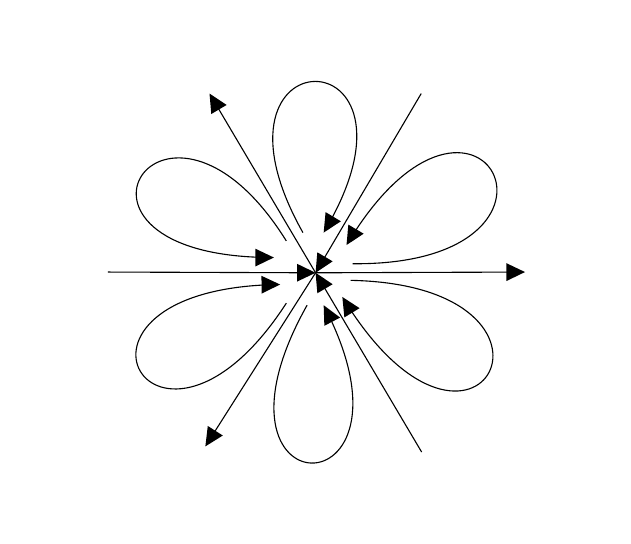
\begin{tikzpicture}[x=0.75pt,y=0.75pt,yscale=-1,xscale=1]
%uncomment if require: \path (0,235); %set diagram left start at 0, and has height of 235

%Straight Lines [id:da7014467597216401] 
\draw    (334,128.64) -- (431.9,128.29) ;
\draw [shift={(434.9,128.28)}, rotate = 539.79] [fill={rgb, 255:red, 0; green, 0; blue, 0 }  ][line width=0.08]  [draw opacity=0] (8.93,-4.29) -- (0,0) -- (8.93,4.29) -- cycle    ;
%Straight Lines [id:da7937079638414151] 
\draw    (334,128.64) -- (284.43,44.86) ;
\draw [shift={(282.9,42.28)}, rotate = 419.39] [fill={rgb, 255:red, 0; green, 0; blue, 0 }  ][line width=0.08]  [draw opacity=0] (8.93,-4.29) -- (0,0) -- (8.93,4.29) -- cycle    ;
%Straight Lines [id:da5652322657720215] 
\draw    (334,128.64) -- (282.51,209.74) ;
\draw [shift={(280.9,212.28)}, rotate = 302.40999999999997] [fill={rgb, 255:red, 0; green, 0; blue, 0 }  ][line width=0.08]  [draw opacity=0] (8.93,-4.29) -- (0,0) -- (8.93,4.29) -- cycle    ;
%Straight Lines [id:da49795176320656886] 
\draw    (384.9,42.28) -- (335.52,126.05) ;
\draw [shift={(334,128.64)}, rotate = 300.51] [fill={rgb, 255:red, 0; green, 0; blue, 0 }  ][line width=0.08]  [draw opacity=0] (8.93,-4.29) -- (0,0) -- (8.93,4.29) -- cycle    ;
%Straight Lines [id:da9443327330326834] 
\draw    (233.9,128.28) -- (331,128.63) ;
\draw [shift={(334,128.64)}, rotate = 180.21] [fill={rgb, 255:red, 0; green, 0; blue, 0 }  ][line width=0.08]  [draw opacity=0] (8.93,-4.29) -- (0,0) -- (8.93,4.29) -- cycle    ;
%Straight Lines [id:da7066291127526734] 
\draw    (385.1,215) -- (335.53,131.22) ;
\draw [shift={(334,128.64)}, rotate = 419.39] [fill={rgb, 255:red, 0; green, 0; blue, 0 }  ][line width=0.08]  [draw opacity=0] (8.93,-4.29) -- (0,0) -- (8.93,4.29) -- cycle    ;
%Curve Lines [id:da8961728852679585] 
\draw    (351.9,124.28) .. controls (472.29,125.27) and (412.51,10.81) .. (349.84,113.71) ;
\draw [shift={(348.9,115.28)}, rotate = 300.82] [fill={rgb, 255:red, 0; green, 0; blue, 0 }  ][line width=0.08]  [draw opacity=0] (8.93,-4.29) -- (0,0) -- (8.93,4.29) -- cycle    ;
%Curve Lines [id:da6878104068351576] 
\draw    (327.9,109.28) .. controls (273.17,12.15) and (394.67,12.65) .. (338.76,107.83) ;
\draw [shift={(337.9,109.28)}, rotate = 300.98] [fill={rgb, 255:red, 0; green, 0; blue, 0 }  ][line width=0.08]  [draw opacity=0] (8.93,-4.29) -- (0,0) -- (8.93,4.29) -- cycle    ;
%Curve Lines [id:da6213553894464128] 
\draw    (319.9,113.28) .. controls (261.19,19.13) and (195.56,120.63) .. (312.13,121.27) ;
\draw [shift={(313.9,121.28)}, rotate = 539.81] [fill={rgb, 255:red, 0; green, 0; blue, 0 }  ][line width=0.08]  [draw opacity=0] (8.93,-4.29) -- (0,0) -- (8.93,4.29) -- cycle    ;
%Curve Lines [id:da5023612601796306] 
\draw    (319.9,143.28) .. controls (257.21,240.17) and (196.51,136.7) .. (315.1,134.3) ;
\draw [shift={(316.9,134.28)}, rotate = 539.3399999999999] [fill={rgb, 255:red, 0; green, 0; blue, 0 }  ][line width=0.08]  [draw opacity=0] (8.93,-4.29) -- (0,0) -- (8.93,4.29) -- cycle    ;
%Curve Lines [id:da5020349766396639] 
\draw    (329.9,144.28) .. controls (273.18,245.15) and (389.72,245.66) .. (338.68,145.79) ;
\draw [shift={(337.9,144.28)}, rotate = 422.4] [fill={rgb, 255:red, 0; green, 0; blue, 0 }  ][line width=0.08]  [draw opacity=0] (8.93,-4.29) -- (0,0) -- (8.93,4.29) -- cycle    ;
%Curve Lines [id:da4534345213536044] 
\draw    (350.9,132.28) .. controls (469.3,134.65) and (411.49,244.55) .. (347.86,141.84) ;
\draw [shift={(346.9,140.28)}, rotate = 418.73] [fill={rgb, 255:red, 0; green, 0; blue, 0 }  ][line width=0.08]  [draw opacity=0] (8.93,-4.29) -- (0,0) -- (8.93,4.29) -- cycle    ;
\end{tikzpicture}

        \caption{Attraction and repulsion vectors, basins where $p = 3$, $\mu\in\R^{> 0}$}
    \end{figure}
\end{frame}
\begin{frame}{Attraction vectors}
    This intuition is formalized in the following results.
    \newline
    \begin{thm}
        Let $f$ be a holomorphic function as with $\lambda = 1$. Let $z_0$ be such that the sequence $z_n=\iter{f}{n}(z_0)\tendsto 0$ but $\forall n, z_n\ne 0$. Then, for some attraction vector $v_j$ satisfying $v_j^p=-1/(p\mu)$,
        \begin{equation*}
            \lim_{n\tendsto\infty} n^{1/p} z_n = v_j
        \end{equation*}
        i.e. $z_n\sim v_j/n^{1/p}$ asymptotically. $z_n$ is said to tend to 0 \emph{in the direction of $v_j$}.
    \end{thm}
    \begin{cor}
        Let $z_0$ be such that the sequence $z_n=\inviter{f}{n}(z_0)\tendsto 0$ but $\forall n, z_n\ne 0$. Then, for some repulsion vector $v_j$ of $f$ satisfying $v_j^p = 1/(p\mu)$, $z_n\sim v_j/n^{1/p}$.
    \end{cor}
\end{frame}
\begin{frame}{Rotational parabolic points}
    We have sneakily been setting $\lambda = 1$. The following result justifies ``WLOG $\lambda = 1$''.\newline
    \begin{dfn}
        Let $v$ be a complex number.  
        \begin{itemize}
            \item If there exists a sequence $z_n=\iter{f}{n}(z_0)\tendsto 0$ (but $\forall n, z_n\ne 0$) with a subsequence $z_{n_k}$ such that $\arg z_{n_k}\tendsto\arg v$, then $v$ is called an attraction vector for $f$.
            \item If there exists a sequence $z_n=\inviter{f}{n}(z_0)\tendsto 0$ (but $\forall n, z_n\ne 0$) with subsequence $z_{n_k}$ such that $\arg z_{n_k}\tendsto\arg v$, then $v$ is called an repulsion vector for $f$.
        \end{itemize}
    \end{dfn} 
    \begin{thm}
        The attraction vectors of $f$ are the same as the same as those of $\iter{f}{r}$, and their number is a multiple of $r$.
    \end{thm}
\end{frame}
\begin{frame}{Attraction basins}
    \begin{itemize}
        \item A specialized ``directional'' notion of an attraction basin is thus needed for our purposes.
        \item Similarly, the notion of a \emph{petal} acts as a directional notion of a neighbourhood of a fixed point.
    \end{itemize}
\end{frame}
\begin{frame}{Basins and petals}
    \begin{dfn}
        The basin of attraction $\basin_v$ for an attraction vector $v$ is defined as the set of points $z$ such that $\iter{f}{n}(z)\tendsto 0$ in the direction of $v$. The immediate basin of attraction $\basin_v^0$ is defined as the unique connected component of $\basin_v$ that is closed under $f$.
    \end{dfn}
    \begin{dfn}
        Where $f$ is injective on some neighbourhood $\nhd$ of its fixed point, an open set $\petal \subseteq \nhd$ is called an attracting petal for $f$ along attraction vector $v$ if 
        \begin{enumerate} 
            \item $\petal$ is closed under $f$.
            \item $\petal\subseteq\basin_v$
            \item Any orbit $\iter{f}{n}(z_0)$ converging to 0 along $v$ is eventually in $\petal$. 
        \end{enumerate}
    \end{dfn}
\end{frame}
\begin{frame}{Basins and petals}
    Basic expected results on attraction basins and neighbourhoods transfer to our new definitions.
    \begin{lem}
        The attraction basin is open.
    \end{lem}
    \begin{lem}
        The basins of attraction $\basin_v$ are contained in the Fatou set of $f$, while their boundaries $\partial\basin_v$ are contained in the Julia set.
    \end{lem}
    \begin{lem}
    Where $f$ is a non-linear rational map with parabolic fixed point 0 and multiplier $\lambda = 1$: 
        \begin{enumerate}
            \item each immediate basin of 0 contains at least one critical point of $f$.
            \item each basin contains exactly one petal $\petal_\mathrm{max}$ that maps injectively onto some right half-plane under $\linT$ and is maximal with respect to this property. 
            \item $\petal_\mathrm{max}$ has at least one critical point of $f$ on its boundary.
        \end{enumerate}
    \end{lem}
\end{frame}
\begin{frame}{Abel linearization}
    \begin{itemize}
        \item $\linT(f(z))=\linT(z)$ is \emph{not} a local homeomorphism!
        \item Better idea to find a linearization: take inspiration from the ``inherent structure on the petal''. $\linT(f(z))=\linT(z)+1$.
    \end{itemize}
    \begin{thm}[Parabolic linearisation theorem]
        Given an attracting or repelling petal $\petal$, there exists a unique (up to composition on the left with translation) conformal embedding $\linT:\petal\to\C$ called a Fatou co-ordinate on $\petal$ such that, for all $z\in\petal\cup {f}\inv(\petal)$, we have:
        \begin{equation*}
            \linT(f(z))=\linT(z)+1
        \end{equation*}
    \end{thm}
\end{frame}
\begin{frame}{Abel linearization}
    \begin{itemize}
        \item Does not immediately suffice for a normal form
        \item Can ``paste'' linearization of each petal together -- Ecalle-Voronin classification
    \end{itemize}
\end{frame}